Við höfum komist að því hvernig búa má til töflur sem vísa hver í aðra. Við höfum líka komist að því hvernig ná má í upplýsingar úr einni töflu.

Nú skulum við líta á hvernig búa má til skipanir sem velja upplýsingar úr fleiri en einni töflu. Til þess þurfum við að læra hvernig stækka má \verb|FROM| klausuna svo að hún geti meðhöndlað margar töflur.
\section{Nöfn dálka}
Áður en lengra er haldið skulum við skoða betur dálitla ónákvæmni sem við höfum sætt okkur við hingað til.

Þegar við höfum vísað í dálk hefur okkur dugað að skrifa einfaldlega nafn hans. Við höfum ekki séð mikið að því að skrifa \verb|WHERE| klausur á borð við \verb|WHERE numer = 11|.

Þetta verður hins vegar erfiðara þegar við vinnum með margar töflur í einu. Hvað ef við erum að vinna með tvær töflur þar sem báðar töflurnar eru með dálk sem heitir \verb|numer|?

Til að passa upp á að gagnagrunnskerfið viti hvaða dálk við eigum við þurfum við oft að taka fram í hvaða töflu dálkurinn sem við erum að nefna er. Þetta er gert með því að skipta út nafninu á dálkinum fyrir ``fullt nafn'' hans. Til að fá fullt nafn dálks skrifum við fyrst nafn töflunnar sem hann er í, svo punkt, svo nafn dálksins. Þannig má vísa í dálkinn \verb|a| í töflunni \verb|A| með því að skrifa \verb|A.a|.

Notkun á fullu nafni dálks má sjá á sýnidæmi \ref{sql:k6d1-fullt-nafn}.

\begin{example}
\caption[Fullt nafn dálks]{Tvær \emph{SELECT} skipanir sem gera það sama - velja auðkenni áfanga úr áfangatöflunni þar sem raðnúmer línunnar er $1$. Munurinn er sá að í seinni skipuninni er tekið fram í hvaða töflu dálkurinn \emph{numer} er.}
\label{sql:k6d1-fullt-nafn}
\centering
\sql{sql/k6d1-fullt-nafn.sql}
\end{example}

\subsection{Að endurnefna - AS}
Það að vinna með heiti getur verið þreytandi. Til að vinna með dálka og töflur undir öðru nafni má nota lykilorðið \verb|AS|. Þetta býr til ``aukanafn''\footnote{e. \emph{alias}} fyrir fyrirbrigðið sem unnið er með. Gamla nafninu er ekki breytt í gagnagrunnskerfinu, \verb|AS| býr bara til nýtt nafn til að nota tímabundið.

Sjá má endurnefndan dálk á sýnidæmi \ref{sql:k6d2-nytt-nafn}.

\begin{example}
\caption[Endurnefning]{Endurnefning dálks. Dálkurinn \emph{audkenni} mun birtast sem \emph{afangi} í niðurstöðum þessarar skipunar.}
\label{sql:k6d2-nytt-nafn}
\centering
\sql{sql/k6d2-nytt-nafn.sql}
\end{example}

\section{Að velja úr meira en einni töflu - JOIN}
Til að segja hvaðan upplýsingarnar sem við ætlum að vinna með í \verb|SELECT| skipun eiga að koma notum við \verb|FROM| klausu.

Hingað til hefur \verb|FROM| klausan ekki innihaldið annað en orðið \verb|FROM| og nafnið á töflunni. Þetta er villandi einfalt. Rifjum upp hvað við sögðum þegar við kynntumst \verb|FROM| klausunni fyrst (undirkafli \ref{undirkafli:from}):
\begin{quote}
\emph{FROM klausa lýsir því hvaðan upplýsingar koma.}
\end{quote}
Þessi lýsing getur innihaldið meira en eina töflu. Almennt séð myndar \verb|FROM| klausan sem sagt \emph{mengi} upplýsinga sem hægt er að vinna með.

Til að skilgreina mengi sem tekur upplýsingar sínar úr tveimur eða fleiri töflum bætum við lykilorðinu \verb|JOIN| (ásamt fleiri lykilorðum) við \verb|FROM| klausuna.

\subsection{INNER JOIN}
\verb|INNER JOIN| er sú leið sem langmest er notuð til að ná upplýsingum úr mörgum töflum. 

Til að skilja \verb|INNER JOIN| betur skulum við skoða aftur hvernig töflur voru tengdar saman með aðkomulyklum (undirkafli \ref{undirkafli:adkomulyklar}).
Aðkomulyklar tengja töflur saman með því að halda utan um gögn sem eru sameiginleg í tveimur töflum. \verb|INNER JOIN| nýtir sér þessi sameiginlegu gögn til að smíða eitt stórt mengi sem vinna má með.

Lítum á mynd \ref{mynd:inner-join}.

\begin{figure}
\caption[INNER JOIN]{Sýnir hvernig \emph{SELECT} skipun með \emph{INNER JOIN} velur einungis þær línur úr töflunum $A$ og $B$ sem dálkarnir $numerA$ og $numerB$ eiga sameiginlegar.}
\label{mynd:inner-join}
\centering
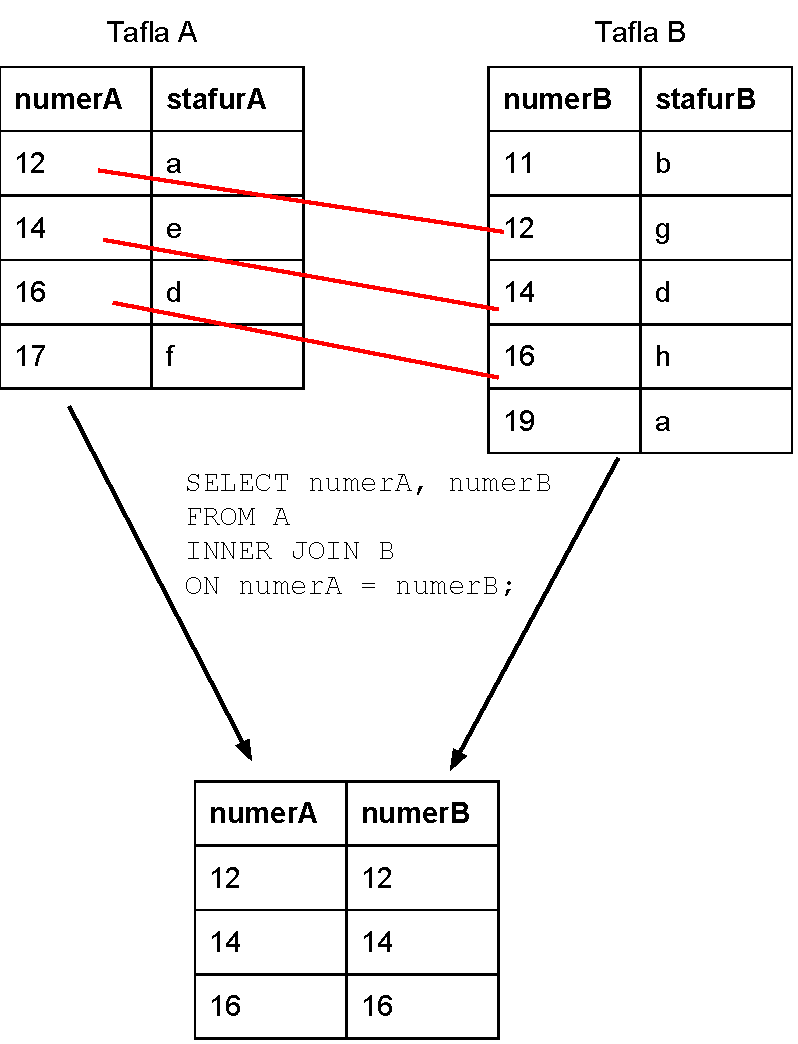
\includegraphics[width=\linewidth]{myndir/inner-join}
\end{figure}

Þar má sjá gildi í tveimur töflum borin saman. Þessi samanburður á sér stað í \verb|ON| hluta skipunarinnar. Hann er líkur samanburði í \verb|WHERE| klausu, en hefur það sérstaka hlutverk að bera saman línur í tveimur mismunandi töflum.\footnote{Venjulega er þetta $=$-samanburður, til að finna þær línur sem eru \emph{eins} í báðum töflum.}

Fyrir utan það að \verb|FROM| klausan er stærri, þá virkar \verb|SELECT| skipun sem velur úr fleiri en einni töflu alveg eins og \verb|SELECT| skipun sem vinnur bara með eina töflu. Hægt er að velja hvaða dálk úr töflunum tveimur sem er.

Sjá má raunverulegri notkun á \verb|INNER JOIN| á sýnidæmi \ref{sql:k6d3-inner-join}.

\begin{example}
\caption[INNER JOIN]{\emph{SELECT} skipun sem velur úr töflunum \emph{Fog} og \emph{Afangar}. Niðurstöðurnar má sjá á mynd \ref{mynd:nidurstada-join}.}
\label{sql:k6d3-inner-join}
\centering
\sql{sql/k6d3-inner-join.sql}
\end{example}

\begin{figure}
\caption[INNER JOIN niðurstaða]{Niðurstaða \emph{SELECT} skipunarinnar í dæmi \ref{sql:k6d3-inner-join}. }
\label{mynd:nidurstada-join}
\centering
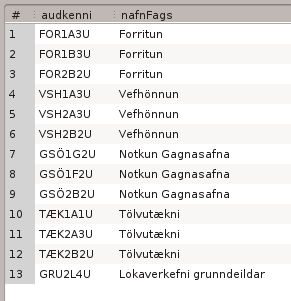
\includegraphics{myndir/workbench-nidurstada-join}
\end{figure}

Hægt er að tengja saman meira en tvær töflur með því að skrifa mörg \verb|JOIN| í sömu \verb|FROM| klausunni. Sjá sýnidæmi \ref{sql:k6d4-tvofalt-join}.

Þegar valið er úr mörgum töflum má líta á það sem svo að sífellt sé verið að stækka það mengi sem valið er úr, eina töflu í einu. Passa þarf upp á að tenging sé á milli allra taflanna sem taldar eru upp. Lína þarf að uppfylla öll skilyrðin í \verb|ON| hlutum skipunarinnar til að geta birst í niðurstöðunum.

\begin{example}
\caption[INNER JOIN]{\emph{SELECT} skipun sem velur nöfn hópa, hvaða áföngum hóparnir tilheyra og hver kennir þá, úr töflunum \emph{Hopar}, \emph{Afangar} og \emph{Starfsmenn}.}
\label{sql:k6d4-tvofalt-join}
\centering
\sql{sql/k6d4-tvofalt-join.sql}
\end{example}

\subsection{ÖNNUR JOIN}
Til að skilja \verb|JOIN| á milli tveggja taflna er gott að hugsa um töflurnar sem verið er að tengja saman sem mengi. Það að finna \verb|INNER JOIN| af töflunum er þá svipað því að finna sniðmengi taflanna - að finna allar línur sem einkennast af því að töflurnar tvær eigi stökin sameiginleg.

\begin{figure}
\caption[Mengi]{Líta má á töflur sem mengi af upplýsingum.}
\label{mynd:join-mengi}
\centering
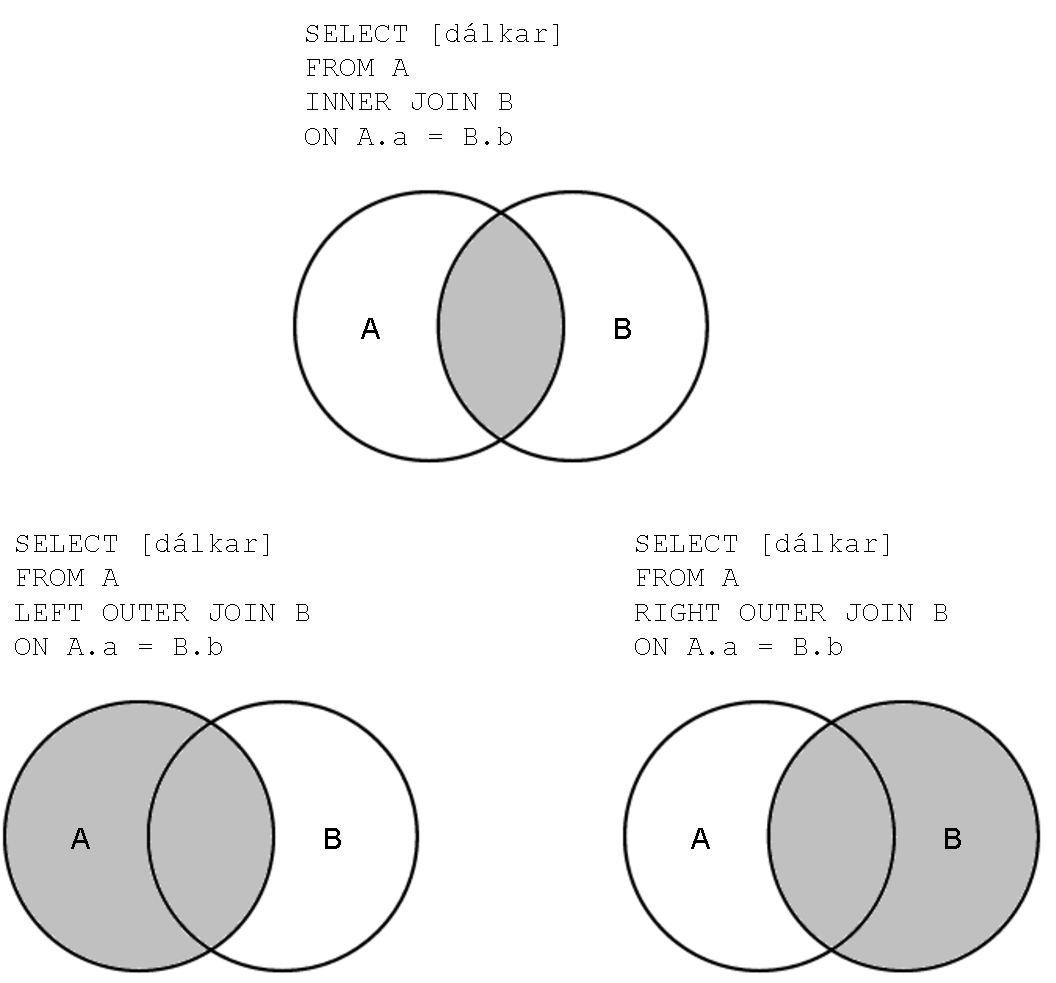
\includegraphics[width=\linewidth]{myndir/join-mengi}
\end{figure}

Þessi mengjahugsunarháttur opnar fyrir möguleikann á fleiri gerðum af \verb|JOIN|um. Svokölluð \verb|OUTER JOIN| geta fundið allar línur í einni töflu ásamt tilsvarandi línu í annarri töflu - ef tilsvarandi lína er til. Í MySQL eru til \verb|LEFT OUTER JOIN| og \verb|RIGHT OUTER JOIN|, sem virka á sama hátt fyrir utan það að þær virka á mismunandi töflur.

Sum gagnagrunnskerfi (en ekki MySQL) hafa líka svokallað \verb|FULL OUTER JOIN|, sem velur allar línur úr tveimur töflum óháð því hvort að stökin eigi eitthvað sameiginlegt.

\section{Undirfyrirspurnir}
\label{undirkafli:undirfyrirspurnir}
Þegar við vinnum með gagnagrunna getum við lent í því að þurfa að nota upplýsingarnar sem við fáum úr fyrirspurn til þess að geta klárað að skrifa aðra fyrirspurn.

Sem dæmi um slíkar aðstæður getum við litið lengst aftur á töflu \ref{tafla:einkunnir}, sem geymir einkunnir nemenda. Í kaflanum sem taflan var sett fram í (kafli \ref{undirkafli:onnur-samsteypufoll}) sáum við dæmi um hvernig við getum skrifað fyrirspurn til að finna meðaleinkunn nemenda í töflunni. En hvað ef við viljum skrifa fyrirspurn sem finnur nöfn þeirra nemenda sem eru hærri en meðaleinkunnin? Ekki dugar að keyra fyrri fyrirspurnina, skrifa niðurstöðuna niður og nota hana í annarri fyrirspurn. Við viljum ekki að fyrirspurnin okkar verði röng ef gögnin í töflunni breytist.

Til að sameina tvær fyrirspurnir af þessum toga breytum við fyrirspurninni sem við þurfum fyrst að fá upplýsingar úr í svokallaða undirfyrirspurn\footnote{e. \emph{subquery}}. Við umlykjum þá fyrirspurn svigum og setjum hana á þann stað í hinni fyrirspurninni sem upplýsingarnar úr innri fyrirspurninni ættu að koma fyrir.

Undirfyrirspurn má sjá á sýnidæmi \ref{sql:k6d5-undirfyrirspurn}.
\begin{example}
\caption[Undirfyrirspurn]{\emph{SELECT} skipun sem notar undirfyrirspurn til að finna þá nemendur sem eru yfir meðaleinkunninni. Undirfyrirspurnin er í \emph{WHERE} klausunni. Undirfyrirspurnin er alltaf keyrð á undan ytri fyrirspurninni.}
\label{sql:k6d5-undirfyrirspurn}
\centering
{\color{red} TODO: Skrifa sýnidæmið sjálft.}
\end{example}
\subsection{Mismunandi hlutverk undirfyrirspurna}
Undirfyrirspurnir eiga það sameiginlegt að skila niðurstöðum sem ytri fyrirspurnin getur nýtt sér og að vera afmarkaðar af svigum. Þar fyrir utan geta þær verið af ýmsum toga.
\begin{itemize}
 \item Undirfyrirspurnir geta skilað einu gildi, dálki af gildum eða heilli töflu af gildum.
 \item Undirfyrirspurnir geta valið gildi úr sömu töflu og ytri fyrirspurnin eða úr öðrum töflum.
 \item Undirfyrirspurnir geta komið fram á mörgum stöðum innan ytri fyrirspurnar, oftast í \verb|WHERE| eða \verb|FROM| klausu.
\end{itemize}
Undirfyrirspurnir geta haft sínar eigin undirfyrirspurnir, það er að segja, undirfyrirspurnir geta verið hver inni í annarri.\footnote{Ef undirfyrirspurnagryfjan er orðin mjög djúp getur verið ástæða til að stoppa og athuga hvort þær séu allar nauðsynlegar.}

Undirfyrirspurnir geta komið fyrir í SQL-skipunum sem ekki eru fyrirspurnir. Þar á meðal eru \verb|INSERT|, \verb|UPDATE| og \verb|DELETE| skipanir.